\section{Introduction} \label{sec:introduction}

\subsection{introduction outline}

\begin{itemize}
\item blurb about AI/ML accelerators (steal from current surface draft?)
\item explain importance of phylogeny data
\item blurb about
\end{itemize}

\subsection{methods outline}

\begin{itemize}
\item reconstruction algorithm overview
\item configuratuons for various WSE-2 and WSE-3 experiments
\item supplement: overview of where to find different parts of code
\end{itemize}

\subsection{results outline}

\begin{itemize}
\item reconstruction quality
   \begin{itemize}
   \item steady vs. tilted vs. hybrid results (Figure \ref{fig:moreno2025testing})
   \item TODO Vivaan fossil reconstruction quality results
   \end{itemize}
\item reconstruction algorithm
   \begin{itemize}
  \item scaling behavior (\Cref{fig:asymptotic,fig:scaling} \citep{singhvi2025scalable})
   \item billion tip reconstruction profile (Figure \ref{fig:billion-tip-time} \citep{singhvi2025scalable})
   \item TODO (supplement) Vivaan reconsteruction quality comparisons vs. naive
   \end{itemize}
\item demonstrations
  \begin{enumerate}
  \item phylogeny topology: purifying vs. adaptive (Figure \ref{fig:on-device}) \citep{moreno2024trackable}
  \item phylogeny trait distribution: preliminary WSE MLS results (Figure \ref{fig:use-case-mls} \citep{moreno2025extending})
  \item cellular automata (WSE3 demo, Figure \ref{fig:use-case-gol}, cite cliff?)
  \end{enumerate}
\end{itemize}

\subsection{conclusion outline}

\begin{itemize}
\item TODO
\end{itemize}

\subsection{Introduction Figures}

\FloatBarrier

% graphic source: https://docs.google.com/presentation/d/11NBuIXM8JQMI2pnPQOirfBzwYOAdVX4sol6ymvlcvqA
\begin{figure}
\begin{minipage}{0.65\linewidth}
\begin{subfigure}{0.55\linewidth}
  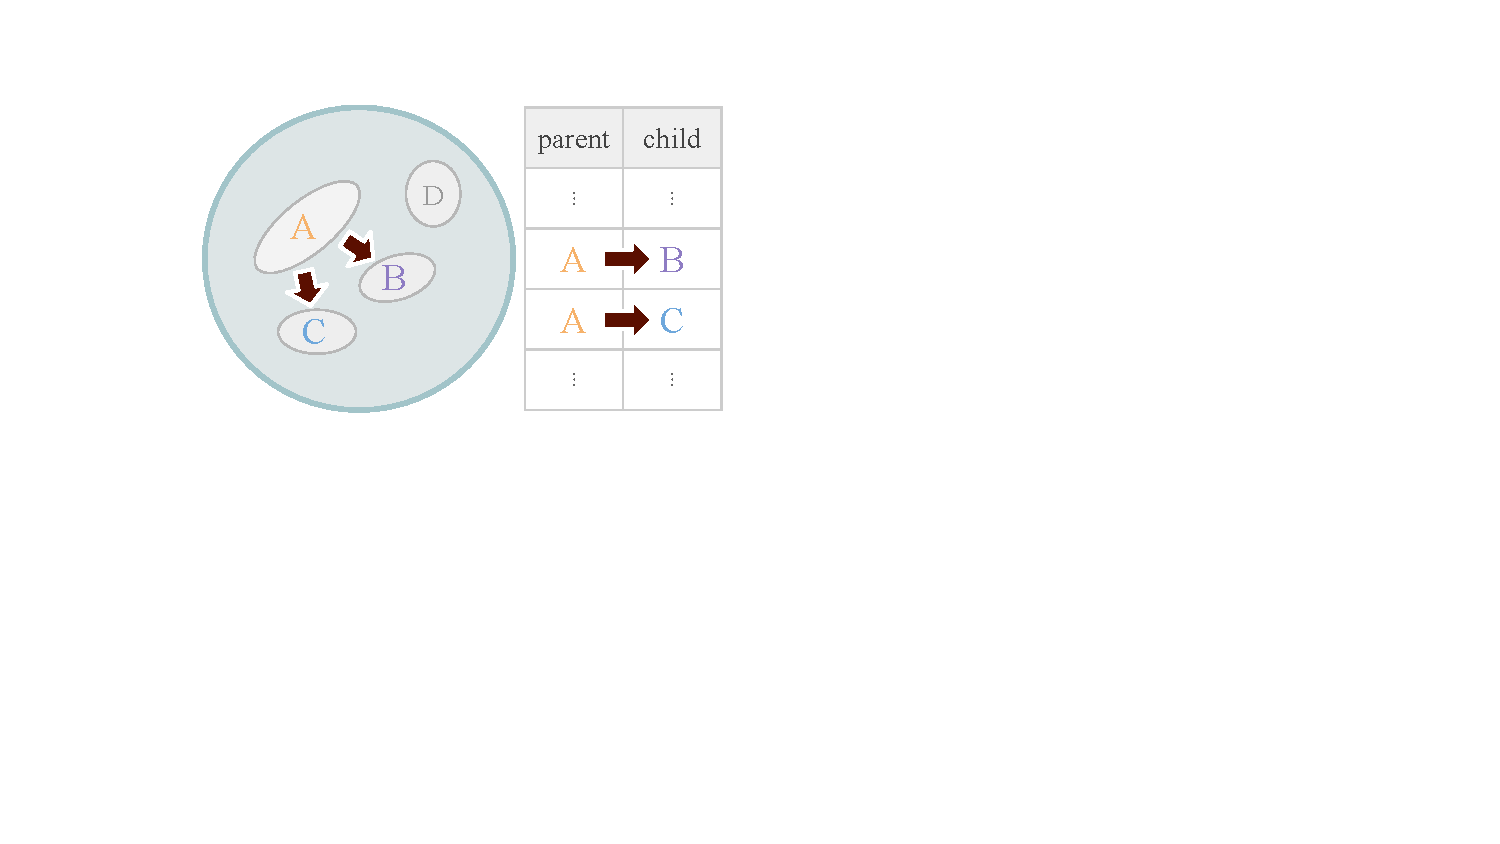
\includegraphics[width=\linewidth]{img/tracking-schematic}
  \caption{\footnotesize tracking approach}
  \label{fig:tracking-vs-reconstruction-schematic:tracking}
\end{subfigure}%
\begin{subfigure}{0.025\linewidth}~\end{subfigure}%
\vrule
\begin{subfigure}{0.025\linewidth}~\end{subfigure}%
\begin{subfigure}{0.35\linewidth}
  \centering
  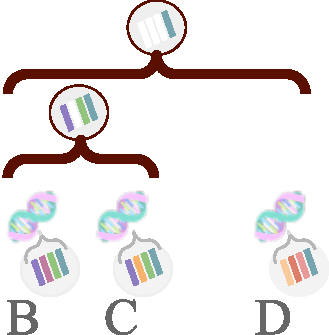
\includegraphics[width=\linewidth]{img/reconstruction-schematic}
  \caption{\footnotesize reconstruction approach}
  \label{fig:tracking-vs-reconstruction-schematic:reconstruction}
\end{subfigure}%
\begin{subfigure}{0.02\linewidth}~\end{subfigure}%
\end{minipage}%
\begin{minipage}{0.35\textwidth}
  \caption{%
  \textbf{Phylogeny tracking versus reconstruction.}
  \footnotesize
  TODO.
  }
  \label{fig:tracking-vs-reconstruction-schematic}
\end{minipage}
\end{figure}


% graphic source https://docs.google.com/presentation/d/10IDom7LfeptDY-rK8ClatmKTfRuEoFrzMhTkaZrDVIA
\begin{figure*}[h]

\centering
\begin{minipage}{0.55\textwidth}

\begin{minipage}{0.41\linewidth}
\centering
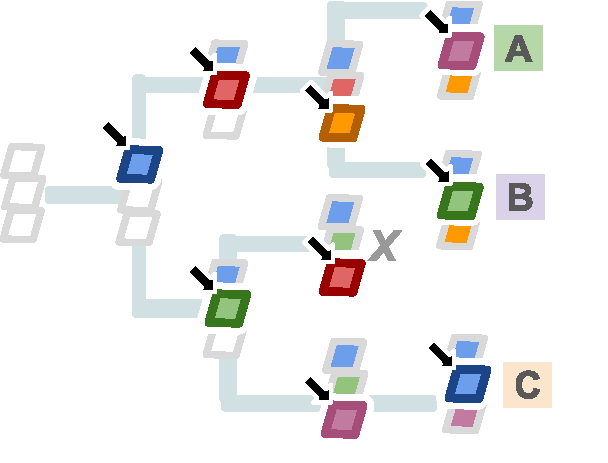
\includegraphics[height=1.1in]{img/hstratschematic-evolve}
\subcaption{evolve}
\label{fig:hstratschematic:evolve}
\end{minipage}%
\vrule
\centering
\begin{minipage}{0.18\linewidth}
~

\includegraphics[height=1.1in]{img/hstratschematic-sample}
\subcaption{sample}
\label{fig:hstratschematic:sample}
\end{minipage}%
\vrule
\begin{minipage}{0.41\linewidth}
\centering
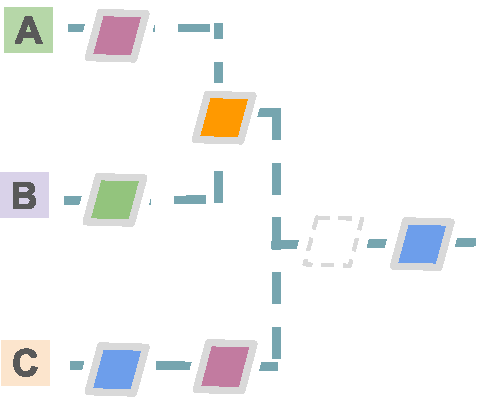
\includegraphics[height=1.1in]{img/hstratschematic-reconstruct}
\subcaption{reconstruct}
\label{fig:hstratschematic:reconstruct}
\end{minipage}
\end{minipage}%
~~
\begin{minipage}{0.43\textwidth}
\caption{%
\textbf{Overview of hereditary stratigraphy.}
\small
At runtime, genomes are annotated with randomly-generated heritable markers (panel \ref{fig:hstratschematic:evolve}).
To maintain fixed-memory footprint, some markers are overwritten.
Genomes of interest are sampled at runtime and from end state (panel \ref{fig:hstratschematic:sample}).
Decoded genome markers enable estimation of evolutionary relatedness (panel \ref{fig:hstratschematic:reconstruct}), subject to error from marker-value collisions and discarded markers.
Adapted from \citet{singhvi2025scalable}.
}
\label{fig:hstratschematic}
\end{minipage}
\end{figure*}


\begin{figure}[h]
\centering
\begin{minipage}{0.62\linewidth}
    \centering
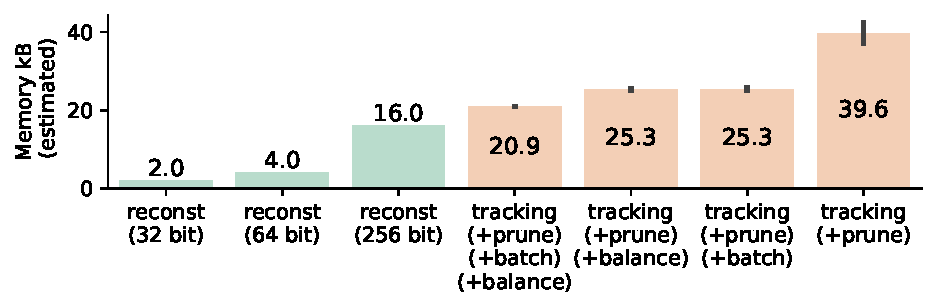
\includegraphics[width=0.95\linewidth]{binder/binder-2025-10-28-trafficsim_msprime.ipynb/binder/teeplots/2025-10-28-trafficsim_msprime/hue=flavor+viz=barplot+x=strategy+y=memory-use-kb+ext=.pdf}
\end{minipage}%
\begin{minipage}{0.38\linewidth}
\caption{%
\textbf{Per-node memory use for phylogeny tracking techniques.}
\footnotesize
Memory estimates for tracking approaches are estimated according to coalescent trees sampled using msprime, to simulate phylogeny migration dynamics across a processor grid.
We assume extinct lineages to be removed from memory through extinction tracking --- meaning that exact records need only be stored for extant lineages (pruning).
We assume unifurcations within the scope of a single PE are collapsed.
For batching optimization, it is assumed that the simulation is halted every 100,000 generations for a clean-up phase where data is offloaded off the chip to free on-chip memory from elapsed history.
For balancing optimization, it is assumed that memory load is shared evenly across the chip so that data capacity is necessary just on behalf of average behavior, not necessarily the most extreme cases requiring a buffer leeway.
Serial direct tracking represents a lower bound on memory usage for a bifurcating phylogeny, which scales as $2B$ population size.
A population size of 512 agents per node is assumed, with demes arranged in a 2D grid and agents migrating between neighboring demes at a rate of 5\%.
Further details on estimation methodology is provided in Section \ref{sec:TODO}.
}
\label{fig:msprime-memory-estimate}
\end{minipage}
\end{figure}


\begin{figure}[h]
\begin{minipage}{0.33\linewidth}
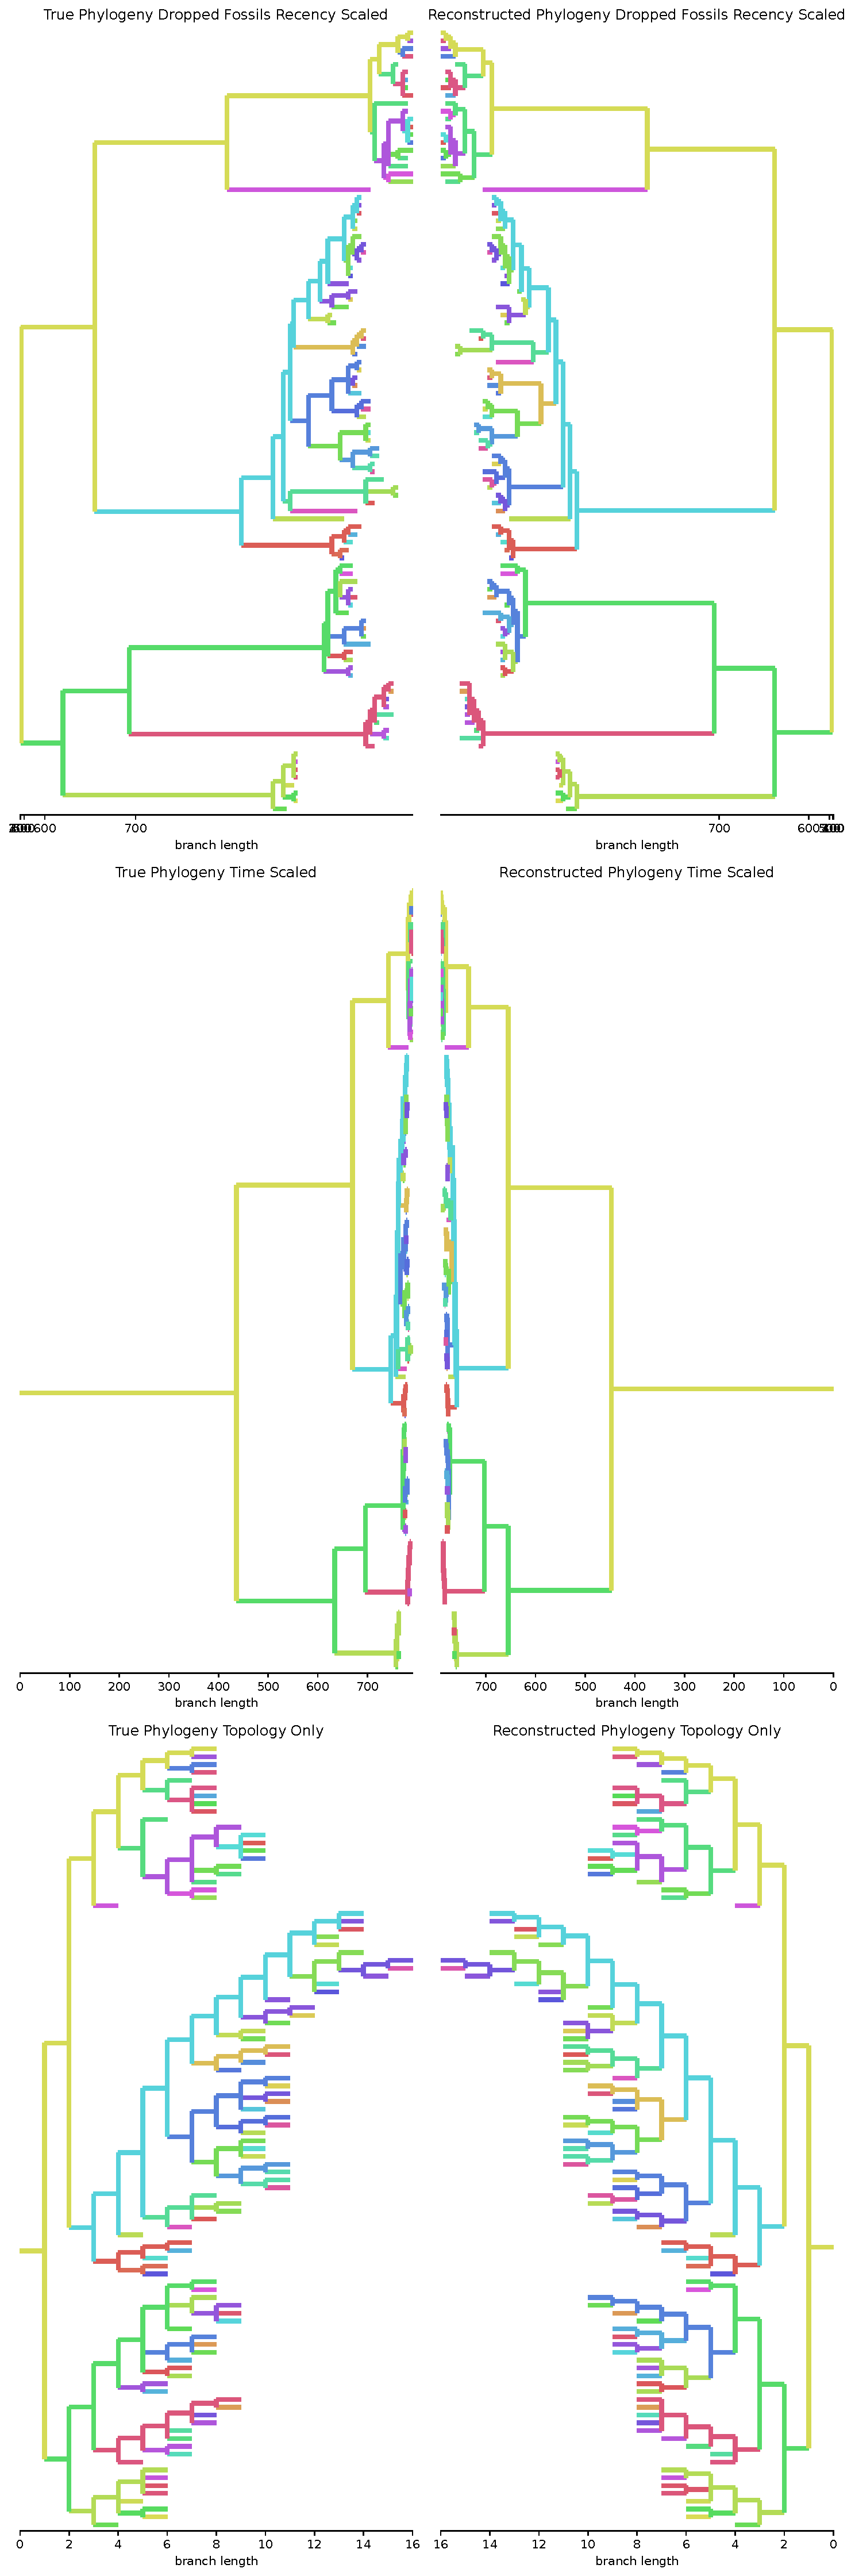
\includegraphics[width=\columnwidth,trim={0 52cm 0 0.8cm},clip]{img/colorclade.pdf}
\end{minipage}%
\begin{minipage}{0.33\linewidth}
\caption{\textbf{Sample comparison of true and reconstructed phylogenies.}
\footnotesize
Generated using a tilted retention policy and a surface of 32 bits. The true phylogeny is on the left and the reconstructed phylogeny is on the right.
Colors are based on a hash from the taxon label for each tip to better facilitate visual comparison. Reconstruction error for this reconstruction was 2.6\%. Visualization created with colorclade \citep{moreno2024colorclade}.
}
\label{fig:colorclade}
\end{minipage}
\end{figure}

